\chapter{学生信息管理系统}
\label{ch:25}

前面各章分别讨论类型、引用、错误和模块，现在把它们放进同一条业务请求：用户登录，取得权限范围，读取或修改教务数据，再把结果显示到页面。功能正确还要求关系完整、失败可说明、服务可启动和数据范围不能越权。

本章对应仓库中真实的学生信息管理工程，包含登录、权限、学生、班级、成绩、科目、教师七个板块。以管理员、教师、学生三类角色串起配置、认证、数据关系、页面与交付；截图和历史验收说明实际环境，不代表所有平台都已运行。

\section{从业务动作确定数据边界}

先从一个可观察动作开始：教师登录后更正自己所教班级的一条成绩。要完成它，需要知道账号是谁、负责哪个班级和科目、学生属于哪里，以及分数是否有效。界面只是入口，这些关系最终都要由后端检查。

管理员负责账号、基础资料与授课授权；教师在授权范围内读写；学生读取本人信息。先确定这些规则，再安排七个板块的页面与路由，可以避免先做出按钮、最后才追补权限。

\begin{center}
\begin{tabular}{lll}
\toprule
板块 & 主要动作 & 权限边界 \\
\midrule
登录 & 登录、退出、修改口令 & 认证成功后才可访问业务 API \\
权限 & 账号角色、启停、授课授权 & 仅管理员写入 \\
学生 & 学号、姓名、年龄、班级和账号关联 & 管理员维护，教师按班级读取，学生只读本人 \\
班级 & 编号与名称 & 管理员维护，其他角色读取关联班级 \\
成绩 & 学生、科目、教师、学期与分数 & 教师只写授课范围，学生只读本人 \\
科目 & 编号与名称 & 管理员维护，其他角色读取关联科目 \\
教师 & 工号、姓名和账号关联 & 管理员维护，其他角色读取关联教师 \\
\bottomrule
\end{tabular}
\end{center}

前端只显示当前角色可用的按钮。真正的数据边界在后端：即使手工发送 HTTP 请求，仍要通过相同校验。

\section{请求经过哪些模块}

\begin{center}
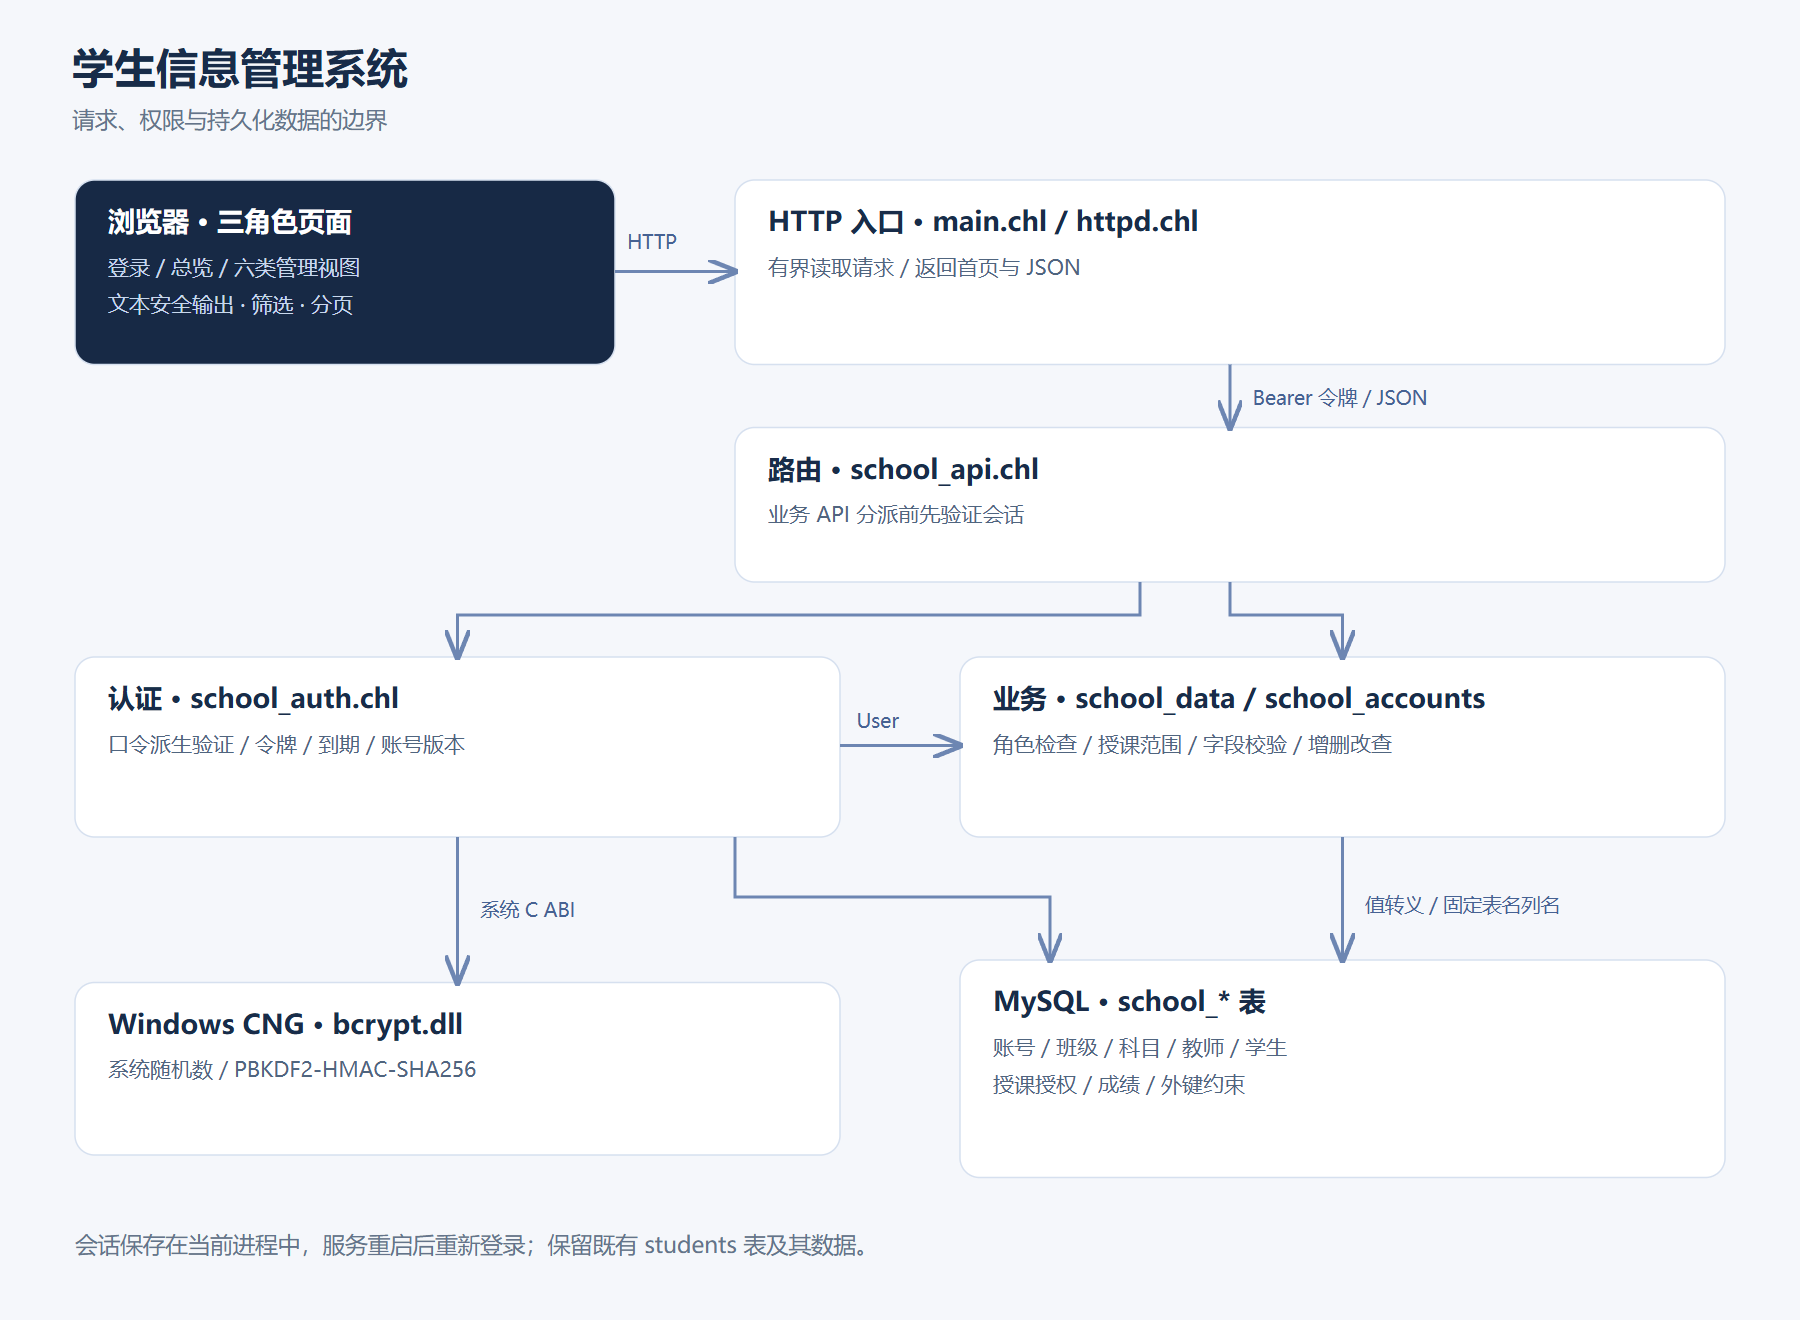
\includegraphics[width=\linewidth,height=0.72\textheight,keepaspectratio]{../images/students-architecture.png}\par
\nopagebreak
系统架构：浏览器、认证、业务数据范围与 MySQL
\end{center}

工程位于 \href{https://github.com/rabbitc999/ChaLi/tree/master/example/students-server}{example/students-server}。main.chl 建立数据库连接并接受 TCP 连接；httpd.chl 读取有大小与时间限制的请求，返回 HTML 或 JSON。school\_api.chl 分派路由，school\_auth.chl 验证会话；school\_data.chl 处理教务表与授课范围，school\_accounts.chl 处理账号与口令。

store.chl 只负责数据库连接配置，api.chl 提供响应和编号解析。crypto.chl 通过系统 C ABI 获取随机数和派生密码摘要。前端保存在 web/index.html，样式和脚本随首页一起提供，不依赖外部 CDN。

\section{配置并启动真实工程}

本章实际验证环境为 Windows x64、外置 LLVM 编译器、MySQL 8 和 Edge。认证示例直接绑定 C:/Windows/System32/bcrypt.dll；其他 Windows 安装位置需要调整声明，其他操作系统需要替换对应系统认证实现，不能只改目标 triple 后声称应用已可部署。

把项目中的 config.example.json 复制为不入库的配置文件，填入有权使用测试库的数据库账号。不要把真实数据库口令写进源码或提交到 Git。

\par
\medskip
\begin{lstlisting}[style=cfg]
{
  "host": "127.0.0.1",
  "user": "school_app",
  "password": "replace-with-local-secret",
  "database": "chali_school",
  "port": 3306
}
\end{lstlisting}
\par
\medskip

\subsection*{代码详解}

host 与 port 定位数据库服务器，和网页服务监听的 8787 端口不是同一用途。user、password 是程序连接 MySQL 的账号凭据，database 选择要使用的库；它们不是浏览器登录学生系统的用户名与口令。

示例中的 password 是占位文字，需替换为本机测试配置，且不能把真实秘密写回书稿或提交。JSON 的键和值都需要正确的引号，port 是数值而不是字符串。连接配置解析成功只证明格式可读，数据库是否存在、账号是否有权限还需启动时实际连接核对。

在仓库根目录运行，三个程序参数依次为端口、网页目录、数据库配置文件：

\par
\medskip
\begin{lstlisting}[style=sh]
chali run example/students-server/src/main.chl -- 8787 example/students-server/web example/students-server/config.local.json
\end{lstlisting}
\par
\medskip

\subsection*{代码详解}

chali run 先编译并执行项目入口，双横线 -- 把编译器选项与程序自己的参数分开。其后三项按顺序交给应用：8787 是网页监听端口，web 路径定位静态页面，最后一个路径定位 MySQL 连接配置；顺序改变就会改变应用解释它们的方式。

这些路径以本命令约定的仓库根工作目录为基准，不能随意切到 src 后照抄。启动后还应观察数据库连接与初始化结果，再打开浏览器登录；只有编译成功并不能证明服务已监听、资源能读取或认证流程可用。不要把数据库的 3306 端口填成网页入口。

浏览器打开 http://127.0.0.1:8787。首次连接空库时建立 school\_ 前缀的表，并在控制台显示随机生成的 admin 初始口令；已有账号时不重置口令。程序不插入业务演示记录。既有 students 表不做迁移或删除。

\section{登录、会话与口令更新}

\begin{center}
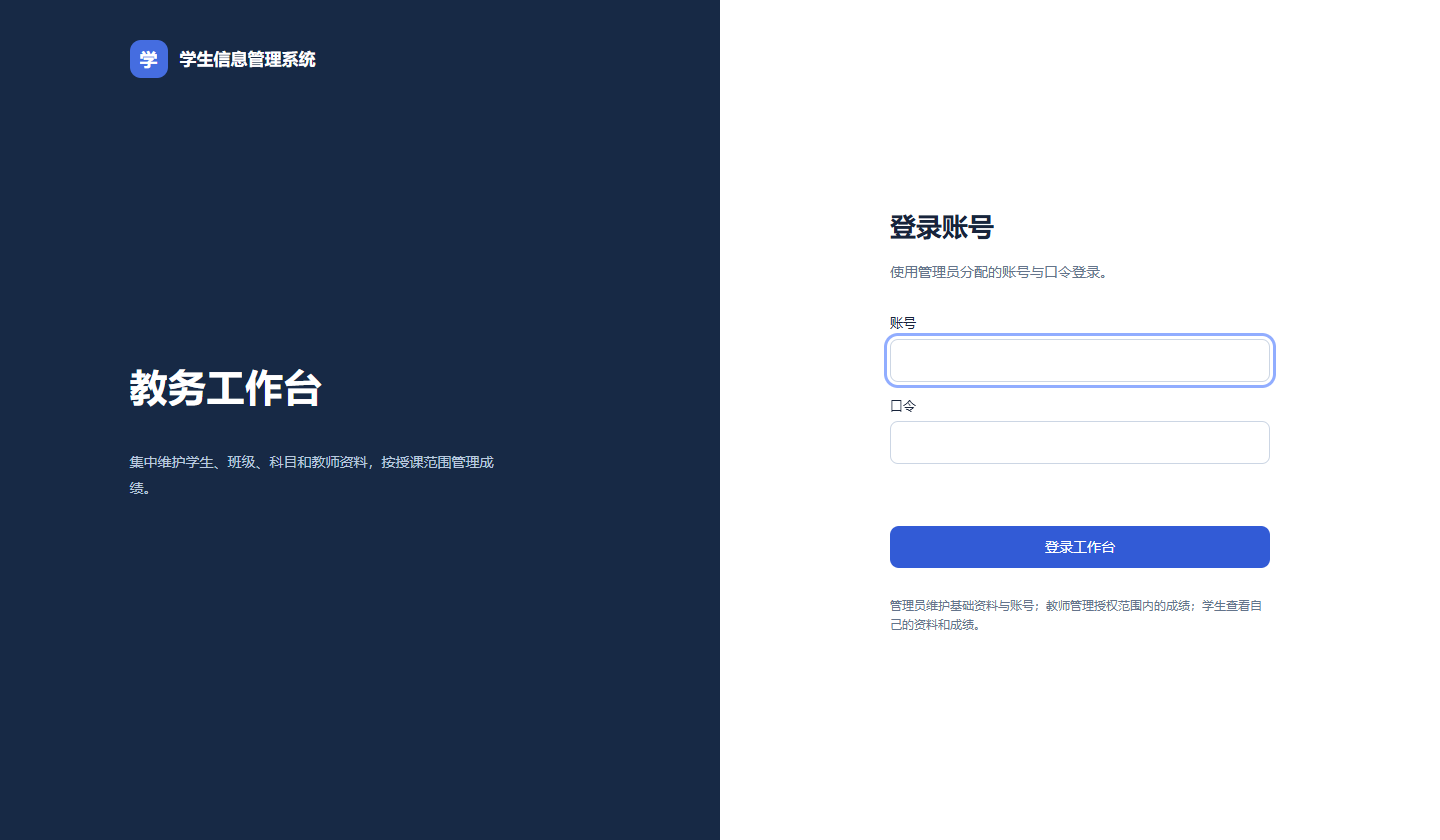
\includegraphics[width=\linewidth,height=0.72\textheight,keepaspectratio]{../images/students-login.png}\par
\nopagebreak
实际运行：登录页面
\end{center}

登录提交账号与口令，服务端用 PBKDF2-HMAC-SHA256 和每个账号独立的随机盐验证摘要，迭代次数为 600000。会话令牌来自系统随机数，保存在服务端内存和当前页面内存中；页面刷新或服务重启后需要重新登录，不写 localStorage。

请求在 Authorization 头中发送 Bearer 令牌。会话有效期为 30 分钟，每次请求重新查询账号启用状态和版本；停用、角色更新或口令修改使旧会话失效。连续五次错误口令会暂时锁定账号 15 分钟，锁定时间用数据库挂钟，进程内会话到期使用单调时钟。

本例默认只监听本机 HTTP。跨机器部署需要在传输层配置 HTTPS，并结合实际并发、账号恢复和审计需求完善运维；本章没有实现密码找回、分布式会话或后台任务。算法说明见 \href{https://learn.microsoft.com/en-us/windows/win32/api/bcrypt/}{Windows CNG} 与 \href{https://cheatsheetseries.owasp.org/cheatsheets/Password_Storage_Cheat_Sheet.html}{OWASP 密码存储说明}。

\section{按关系建立基础资料}

先建立班级和科目，再建立账号、教师与学生资料，最后配置授课授权。账号角色不是姓名字段：教师资料的 user\_id 必须关联教师账号，学生资料必须关联学生账号；未关联账号的人员记录仍可由管理员维护。

\begin{center}
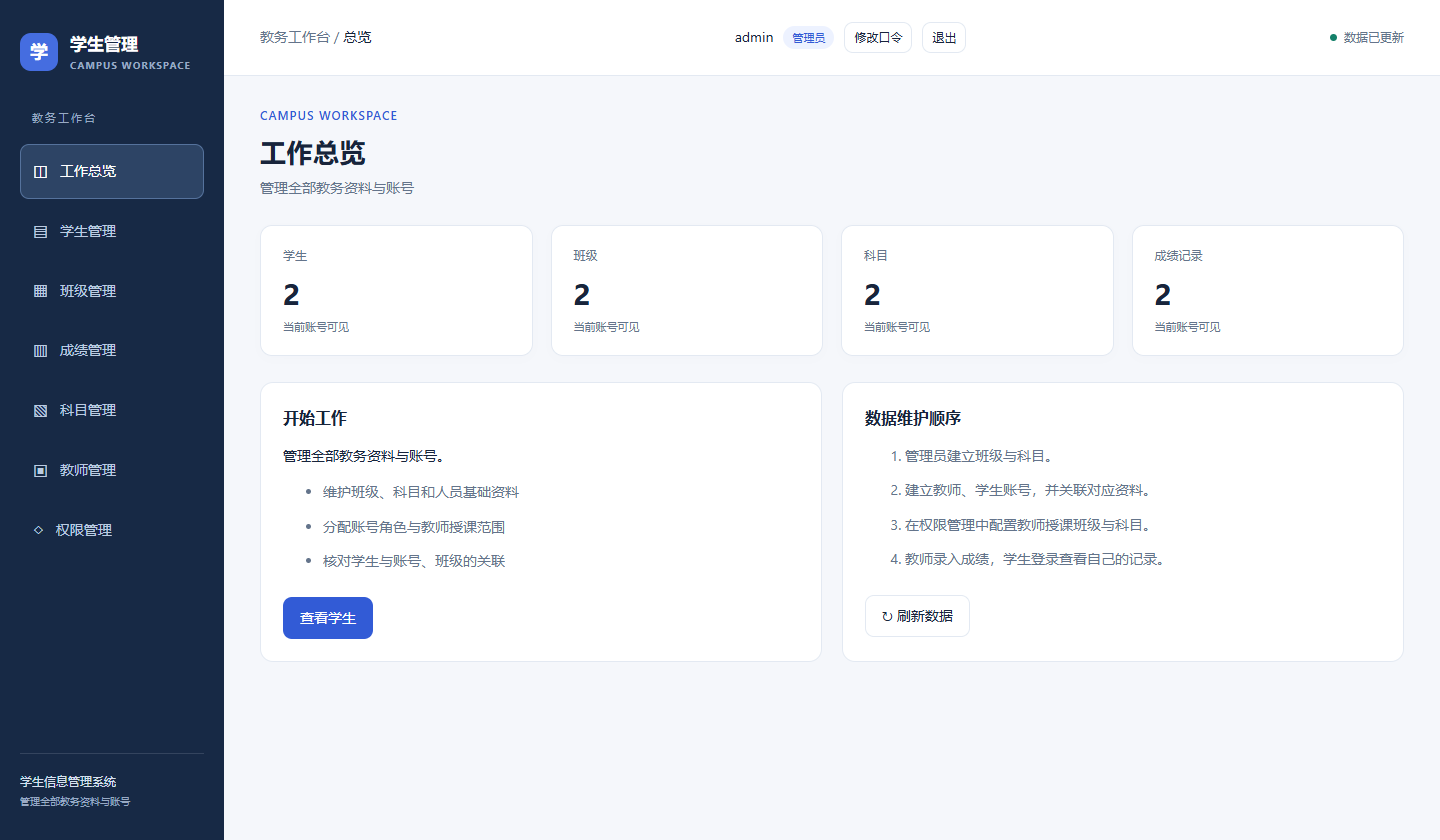
\includegraphics[width=\linewidth,height=0.72\textheight,keepaspectratio]{../images/students-admin-overview.png}\par
\nopagebreak
实际运行：管理员总览，包含两个班级、两名学生和两条成绩
\end{center}

班级编号、科目编号、学号、工号和账号名称分别唯一。学生引用班级，授课授权引用教师、班级和科目，成绩引用学生、科目和教师。外键保护仍被使用的记录；重复编号、无效关联和越界成绩都返回失败结果，页面显示原因而不是宣称保存成功。

\section{授课授权与成绩写入}

\begin{center}
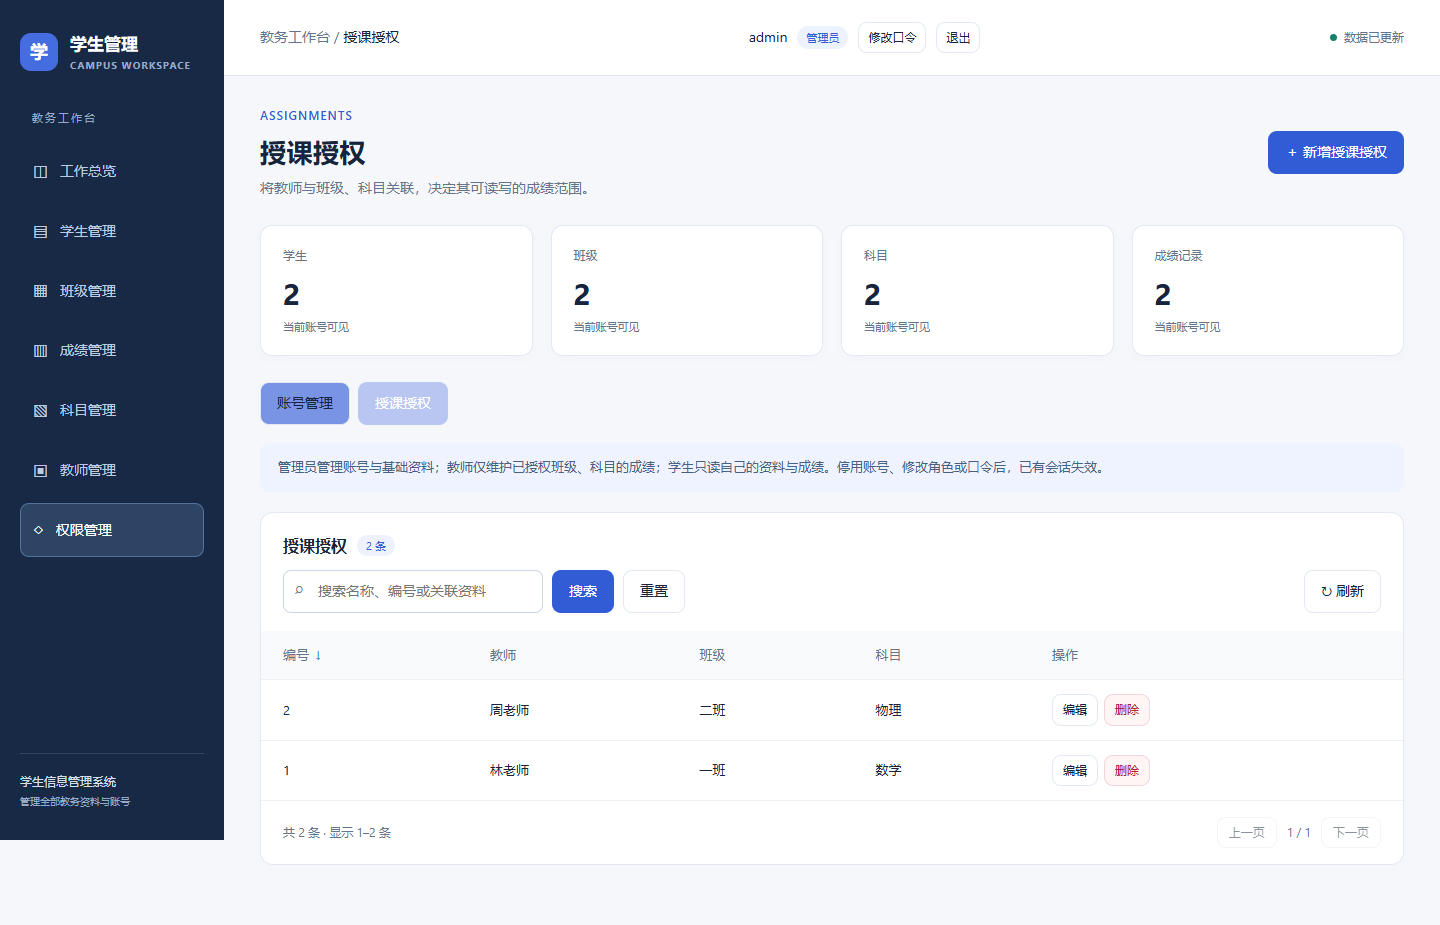
\includegraphics[width=\linewidth,height=0.72\textheight,keepaspectratio]{../images/students-admin-permissions.png}\par
\nopagebreak
实际运行：管理员配置教师、班级与科目的授课授权
\end{center}

一条授课授权由 teacher\_id、class\_id 和 subject\_id 组成。教师写入成绩时，后端检查学生当前班级、科目和所选教师是否存在对应授权，并确认教师账号属于当前登录用户。仅知道另一条成绩的 id 不足以读取或修改它。

\begin{center}
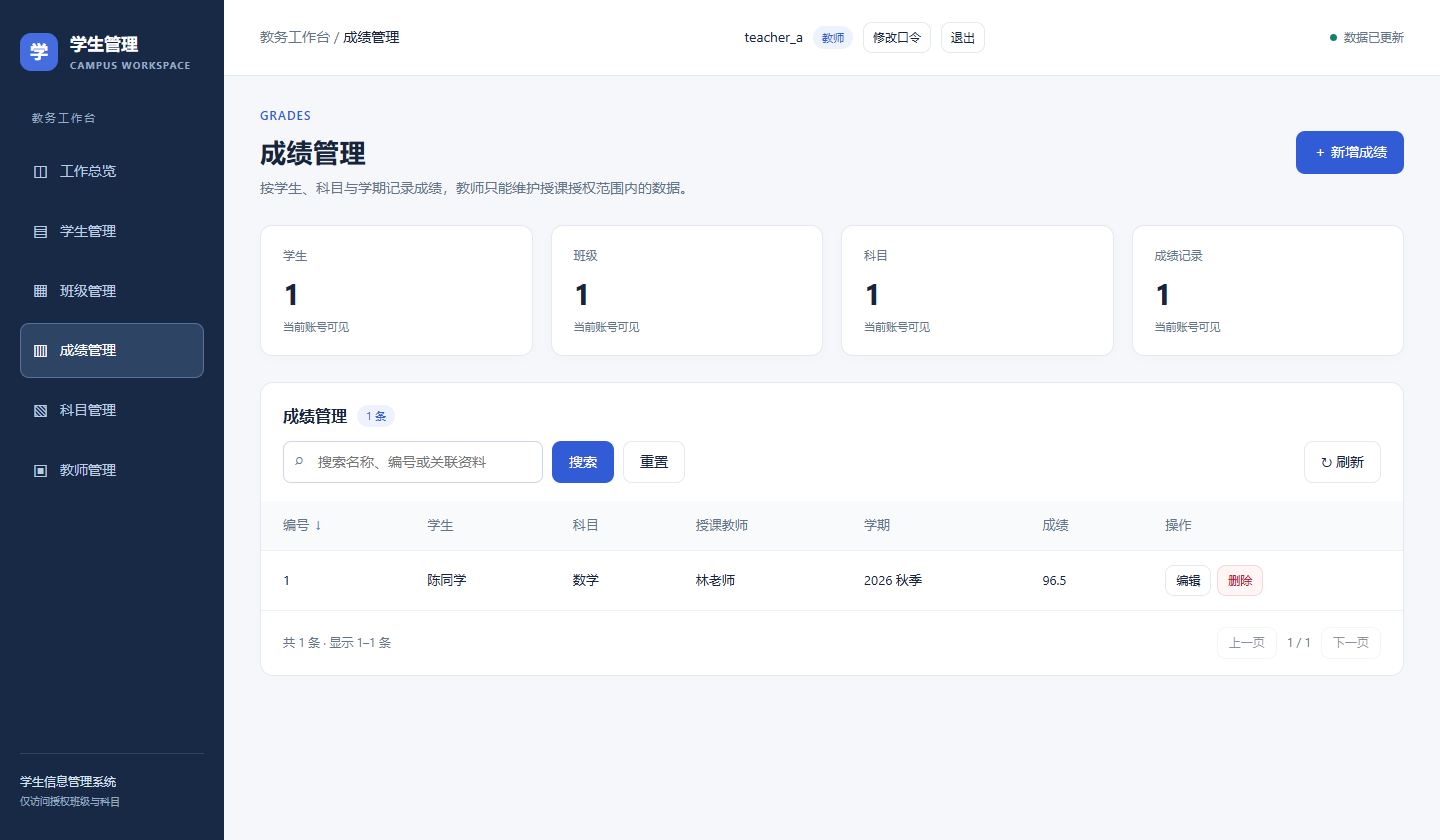
\includegraphics[width=\linewidth,height=0.72\textheight,keepaspectratio]{../images/students-teacher-grades.png}\par
\nopagebreak
实际运行：教师更正自己授权范围内的数学成绩
\end{center}

成绩按学生、科目和学期去重，分数限制在 0–100。PUT 更新即使值与原值相同也视为已存在记录的合法更新，不依赖 MySQL affected=0 推断记录不存在。授课范围变化后权限按当前授权重新计算，既有成绩保留；历史教师与科目仍供对应学生读取名称。

\section{学生只读视图与窄屏布局}

\begin{center}
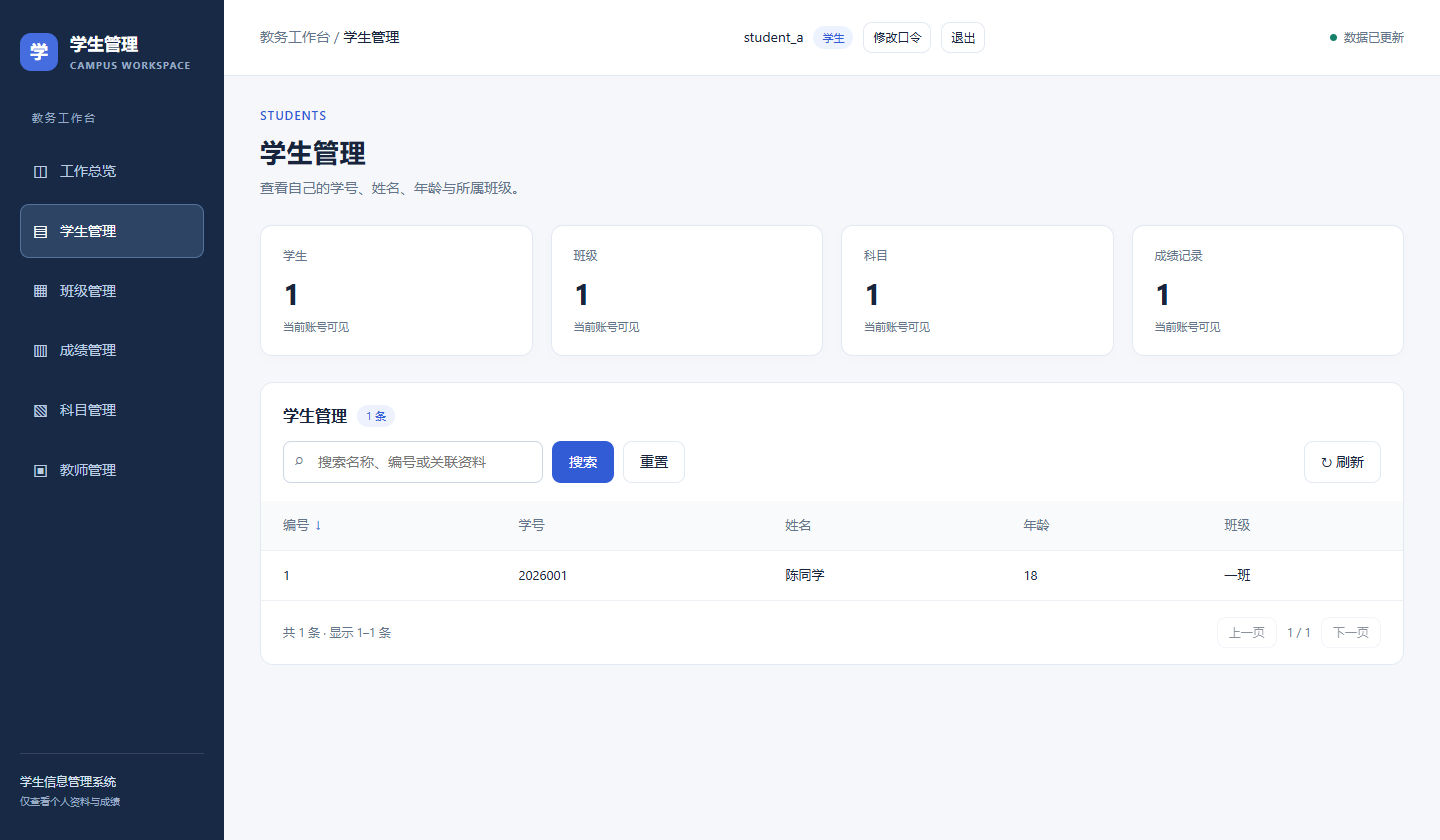
\includegraphics[width=\linewidth,height=0.72\textheight,keepaspectratio]{../images/students-student-students.png}\par
\nopagebreak
实际运行：学生账号只看到自己的学生资料
\end{center}

学生页面没有新增、编辑和删除操作，后端对同样的写请求也返回拒绝。概览统计按当前账号可见数据计算：学生看到的“学生 1”表示自己的可访问记录，不是全校人数。

\begin{center}
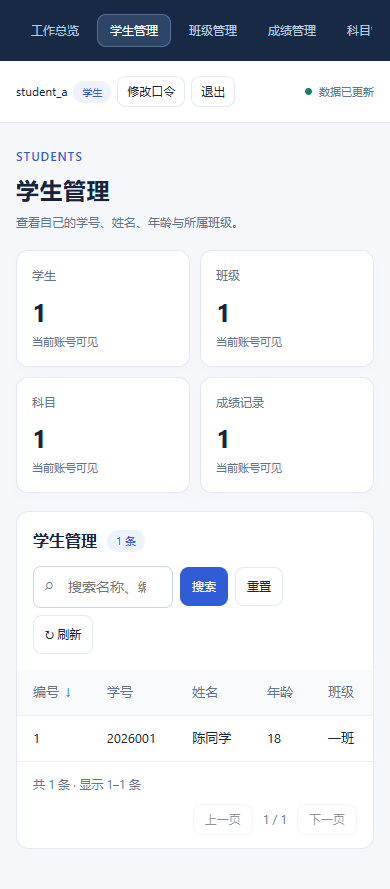
\includegraphics[width=\linewidth,height=0.72\textheight,keepaspectratio]{../images/students-student-mobile.png}\par
\nopagebreak
实际运行：390 像素宽度下的学生页面，导航与表格可在各自区域横向滚动
\end{center}

页面采用统一侧栏、页头、统计卡片、筛选和分页。窄屏把侧栏改为横向导航；表格在容器内部滚动，页面本身不横向溢出。弹窗支持键盘焦点、Escape 和取消，提交期间阻止重复保存。

\section{输入、SQL 和页面输出}

后端只接受固定表名与列名，路径不能变成任意 SQL 标识符。JSON 字段分别检查文本、整数或分数类型，再验证长度、范围及关系。MySQL 接口当前使用 Database.quote 处理文本字面量；不能把 SQLite 的参数化能力当成当前 MySQL 接口已经提供的功能。

前端将用户数据赋给 textContent，而不是将姓名或班级名称拼入 innerHTML。筛选和分页在本次已加载数据中进行，每次列表查询上限为 10000 条；超过上限会返回错误，没有实现面向大数据量的游标分页。

\begin{center}
\begin{tabular}{lll}
\toprule
路由 & 方法 & 含义 \\
\midrule
/api/auth/login & POST & 登录 \\
/api/auth/me & GET & 当前账号 \\
/api/auth/logout & POST & 撤销当前令牌 \\
/api/auth/password & POST & 校验旧口令后更换口令 \\
/api/accounts & GET／POST & 管理员读取或新建账号 \\
/api/accounts/id & PUT／DELETE & 更新或删除账号 \\
/api/students 等业务路径 & GET／POST & 按角色读取列表或创建记录 \\
/api/students/id 等业务路径 & PUT／DELETE & 先检查数据范围，再更新或删除 \\
\bottomrule
\end{tabular}
\end{center}

其余业务路径为 classes、grades、subjects、teachers 和 assignments。错误响应统一带 error 字段。

\section{导出与业务验收}

导出后仍需准备网页目录、数据库配置和 MySQL 客户端依赖。进程内会话不进入数据库备份；备份数据库时同时核对账号关联和业务外键。部署步骤与交叉编译边界见第 24 章。

项目验证使用独立临时数据库，包含有效增删改查、重复键和外键拒绝、三角色数据隔离、教师越权写拒绝、会话撤销及浏览器操作。验证结束关闭服务并删除该测试库，不连接或清空已有业务库。自动验证入口为 \href{https://github.com/rabbitc999/ChaLi/blob/master/tests/students_server.py}{students\_server.py} 和 \href{https://github.com/rabbitc999/ChaLi/blob/master/tests/students_server_ui.py}{students\_server\_ui.py}。

本章截图来自 Windows x64 上运行的真实服务、MySQL 隔离库与 Edge 浏览器。姓名、班级和成绩均为验收数据；图中账号角色和统计范围与实际权限结果对应。

章末番外保留早期单模型反射示例的叙事与技术对照，旧小节编号沿用原文。当前七板块工程采用本章列出的关系表、认证与字段白名单。

\subsection*{小结}

以教师更正成绩为例，把整条链重新走一遍：浏览器提交令牌与数据，服务端确认会话和账号，验证字段与授课范围，再写数据库并形成响应，页面根据真实结果更新。只验证页面按钮或只验证数据库写入，都不能覆盖整条链。

对照前文，结构体组织业务值，枚举与 Result 表达状态，模块组织责任，C ABI 连接系统能力，AOT 决定交付路径。继续扩展时保持这些边界，新增功能附上对应正反例，不把本章的本机验收直接推成任意部署承诺。

\section{习题}

\begin{enumerate}

\item 用管理员建立一名教师、一个班级和一门科目，再配置授权。

\item 尝试用教师令牌修改另一班级的成绩。

\item 停用学生账号后复用其旧令牌。

\item 说明清空浏览器内存、服务重启和数据库备份分别影响什么。

\end{enumerate}

\subsection*{参考解答与验收要点}

\begin{enumerate}

\item 按依赖顺序建立记录，教师账号登录后核对可见范围。

\item 后端返回拒绝，目标记录保持不变；不能只检查按钮隐藏。

\item 旧令牌应被拒绝，因为请求重新检查账号状态和版本。

\item 页面刷新丢失令牌，重启丢失内存会话，数据库备份保留账号和业务记录。

\end{enumerate}

\section{番外：目无全牛}

改写自《庄子·养生主》庖丁解牛。

庖丁为文惠君解学生表。手之所触，肩之所倚，足之所履，膝之所踦，字段霍然向然，奏刀騞然，莫不中反射之会。

文惠君曰：“嘻，善哉！技盖至此乎？寡人不过加了一个班级字段，何以你的建表列、JSON 键、界面清单都跟着变了？”

庖丁释刀对曰：“臣之所好者，结构也，进乎手抄矣。始臣之解表之时，所见无非整段字符串者。三年之后，未尝见整表也。方今之时，臣以元数据遇而不以眼抄，依乎模型，批大隙，导大窾，因其固然。”

“良程序员岁更字段表，抄也；族程序员月更正则，猜也。今臣之模型十九次变更矣，所解接口数千矣，而列名清单若新发于声明。”

文惠君大悦，要把所有用户输入原样拼进 SQL，谓顺其自然。庖丁急拦：“虽然，每至于外部输入，吾见其为难，怵然为戒，视为止，行为迟。值须转义，排序列须核准，校验不容省。”

忽有连接未开，庖丁不下刀；又有影响零行，庖丁留诊断。君问何不假装成功，以免扫兴。庖丁揩刀而藏，答曰：“善哉！臣只会顺着结构解牛，不会顺着报表造牛。”

文惠君曰：“善哉！吾闻庖丁之言，得维护系统焉。”随即又补了一条需求：“顺便支持导出 Excel，应该不复杂吧？”

\subsection*{技术对照}

本章的系统就是把「眼睛」换掉的那个过程：字段清单、建表列、JSON 键不靠手抄，从反射给出的结构里长出来（25.3、25.5），模型改了，派生处自动跟上，刀刃不钝。硬拼 SQL 就像砍骨头——值不过转义、排序字段不过白名单，短期看不出事，缺口都在暗处（25.6）。而「怵然为戒」对应的是失败路径：空连接、超时、脏数据、影响 0 行，每一处都认真对待、留下诊断，程序才经得起长久使用（25.7、25.11）。
